\newchapter{c:feedforward}{Feedforward Results}

This is the introductory text.

\newsection{s:gainScans}{Gain Scans}

\newsection{s:jitterRecord}{Correction at Optimal Gain}

\begin{figure}
  \centering
  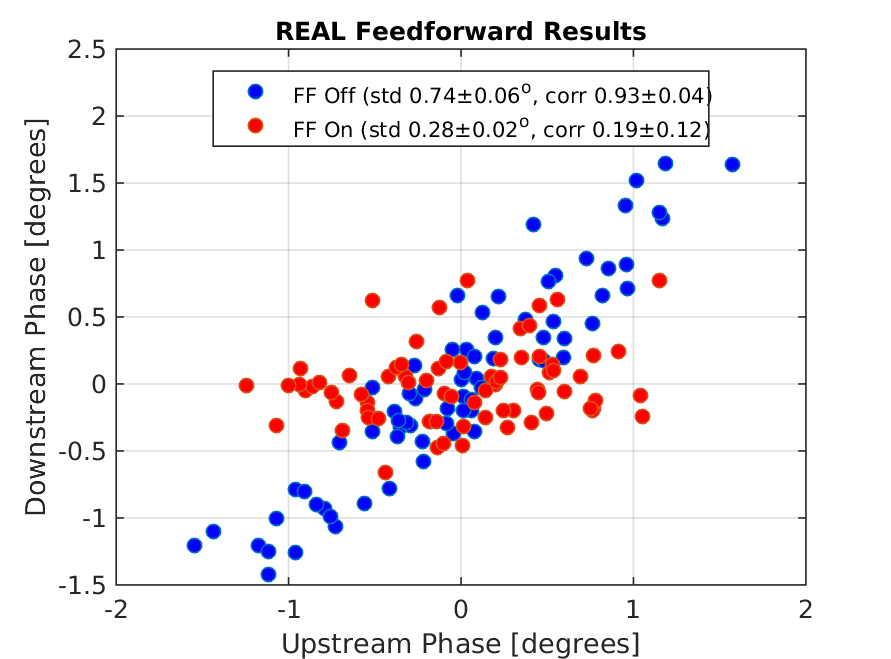
\includegraphics[width=0.45\textwidth]{Figures/BestFF_Real}
  \caption{Mean phase.}
  \label{f:BestFF_Real}
\end{figure}

\begin{figure}
  \centering
  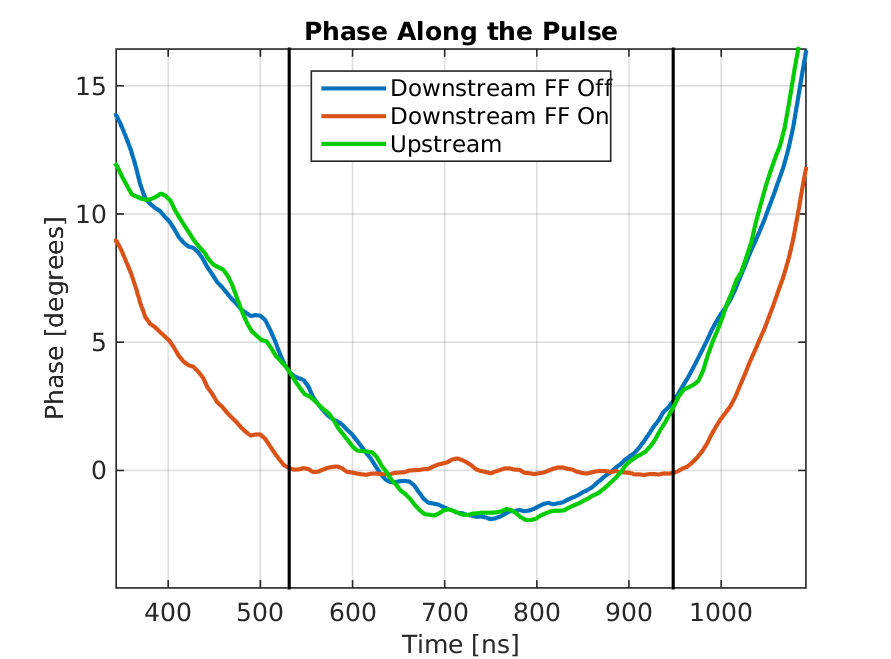
\includegraphics[width=0.45\textwidth]{Figures/BestFF_MeanPhaseAlong}
  \caption{Mean phase along.}
  \label{f:BestFF_MeanPhaseAlong}
\end{figure}

\begin{figure}
  \centering
  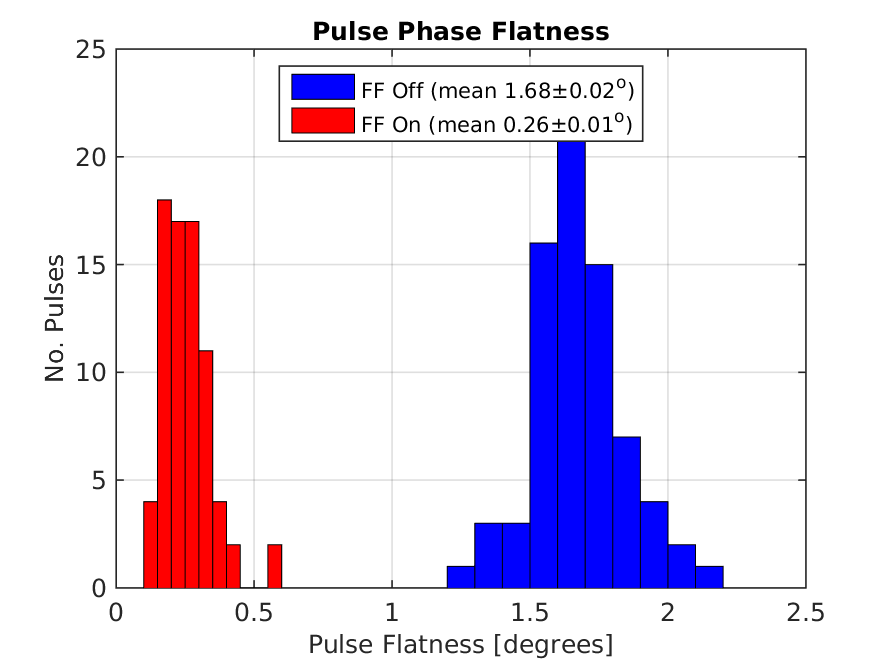
\includegraphics[width=0.45\textwidth]{Figures/BestFF_Flatness}
  \caption{Flatness.}
  \label{f:BestFF_Flatness}
\end{figure}

\newsection{s:simFF}{Simulated PFF Results}

\begin{figure}
  \centering
  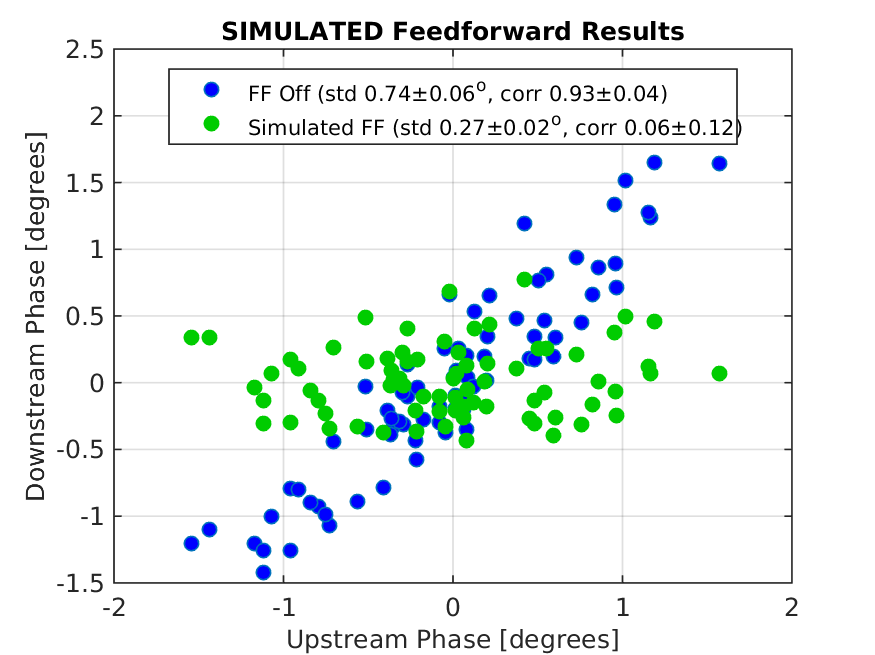
\includegraphics[width=0.45\textwidth]{Figures/BestFF_Simulated}
  \caption{Simulated PFF.}
  \label{f:BestFF_Simulated}
\end{figure}

\newsection{s:longPFF}{Correction on Longer Timescales}

\newsection{s:pffNovelSetups}{Correction with Additional Jitter Source}

\newsection{s:slowCorr}{Slow Correction}





